
\chapter{Audio file formats and steganography techniques}

\begin{multicols}{2}
\section{Introduction}
Sound is the result of a vibration created by a phenomenon that propagates through a transmission environment, ending up getting interpreted by our brain. However since this process happens in the physical world it is entirely analog so it would be impossible to store it on modern day devices which can only understand digital formats. Luckily the fast evolution of computers also brought conversion techniques in order to switch between analog sounds and digital sounds seamlessly, without any noticeable loss to the human ear. Using these methods we have gained the ability to store audio files in a digital format so it was only logical that several different file formats will be created to fit our needs. In this chapter we will discuss in greater detail about how the analog data is actually stored in the digital format and what are the most common extensions used for storing digital audio files.

We mentioned earlier that it is impossible to store analog signals in a digital environment. The solution to this problem is to convert the audio signal which can be represented as a continuous-time function into a discrete-time function using a process called sampling. 

\begin{figure}[H]
    \centering
    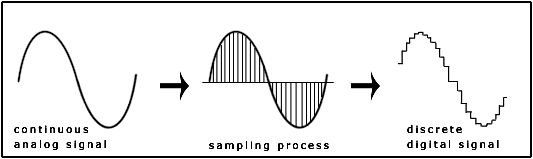
\includegraphics[width=7.7cm,keepaspectratio]{pics/Sampling-of-audio-signal.png}
    \caption{Converting a continuous signal into a discrete one\cite{real_time_audio_steganography}.}
    \label{sampling-graphic-example}
\end{figure}

The sampling process can be observed in figure \ref{sampling-graphic-example}. We can now introduce some new terms that we will use throughout the rest of the chapter:
\begin{itemize}
	\item \textbf{Sampling rate} is the number of samples taken per second, or in other terms, how many discrete values we store for each second of the audio signal. The measurement unit for sampling rate is Hertz (Hz for short) and some of the most common values are 44100, 48000 and some of their multiples.
	\item \textbf{Bit depth} is the number of bits used to store a single sample after having it converted to a discrete value. The most common bit depths are 8, 16, and 24 which allow for 256, 65536, and 16777216 different values. 
	\item \textbf{Audio channel} is the term used to describe the sequence of bytes that represent sampled audio signals. An audio file can have multiple channels to better simulate the sound accuracy and origin in a limited environment. Files with one audio channel are called mono, with two they become stereo and any more channels makes them surround. However, no matter the number of channels, usually all of them are equal in length and the samples from each channel are played simultaneously.
\end{itemize}

In the steganography field, the most common configuration that accepts alterations to the sampled data without losing any noticeable quality is a sampling rate of 44.1kHz with a bit depth of 16 and any number of audio channels, so this the ideal format that we will use throughout the rest of the chapter. The reason why this configuration is favored so much is because of the popularity that came with the invention of CDs and MP3s which used it as a default. Furthermore, any changes made to the sampled data are usually small enough that they will not be noticeable according to the Nyquist-Shannon sampling theorem \cite{Shannon1949}, which is used to compute the condition such that the conversion from a continuous signal to a discrete one will capture all the relevant information. Using the aforementioned theorem and armed with the knowledge that the human physiology enables us to hear audio signals ranging from 20Hz to 20kHz, we can see why the 44.1kHz sampling rate is ideal in audio steganography.

\section{Additional techniques used in audio steganography}
\subsection{Frequency domain steganography}
So far in this thesis we have talked about what can only be classified as spatial domain steganography, like how a pixel of an image is composed of bytes and that altering those byte values in a smart way allows for message embedding or how we can use the file specifications to our advantage and hide information in the file metadata or after the offset where all renderer programs will stop parsing. All of the previous examples deal ony with the spatial domain of the format because they work on the raw bytes and consider each of them to be completely individual and self-sustaining entities that can be altered for steganographic purposes. However, there is another domain that works differently than the spatial one and it is called the frequency domain. In this domain the final representation of the stored data is done by combining the entire range of frequencies into the equivalent signal, usually by using a transform function, the most common being the Fourier transform. The advantage of the frequency domain is that it helps split a signal of any type into clear and distinct sinusoids that are easier to perform complex tasks on. 

In figure \ref{time_vs_frequency_comparison} we can see the differences between the time domain and the frequency domain: the former evolves over time and is highly irregular in most cases(in real world there will never be a perfect sinusoidal signal and will be more similar to the last example), while the latter is easier to manipulate and identify, and through the aforementioned transform functions can be converted back into the time domain.
\begin{figure}[H]
    \centering
    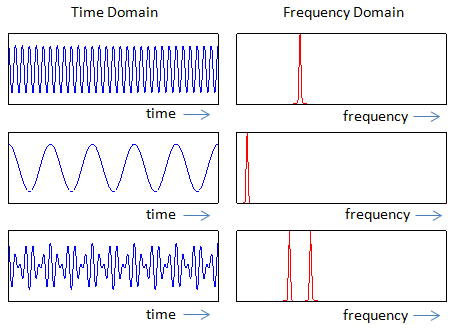
\includegraphics[width=7.7cm,keepaspectratio]{pics/audio_chapter/time_vs_frequency_domains.png}
    \caption{Time domain vs. frequency domain.}
    \label{time_vs_frequency_comparison}
\end{figure}

In the digital images world, the frequency domain is used to know by how much pixels variate from one another, in other words, the rate with which the pixels change. The most common format used for images that takes advantage of the frequency domain is JPEG, but since it is the only known format which uses sinusoids when rendering the image, the authors chose not to include it since the steganographic surface was somewhat limited. However, in the digital audio world every sound will eventually become an analog signal before reaching our ears so it is more common to see algorithms developed specifically for this format that involve altering the sinusoids to our advantage.

For example, we have the technique described in the article Frequency Domain Steganography by Ganier et al.\cite{ganier_hollman_rosser_swanson} where they showcase the most basic way of embedding an audio file within another audio file: since both files have audio signals that are stored as frequencies, it is possible to "compress" the signals so that they only occupy a very specific frequency range and hide the message within the inaudible frequencies of the carrier, a much trivial task when not working in the time domain. This method takes advantage of the human physiology we mentioned earlier and achieves a high rate of success. Similar work has been done by Westfeld et al. \cite{dsss_sstv} where they took the audio signal generated by the Slow Scan Television(SSTV) and embedded it into another carrier audio signal without any audible noise being generated that could alert intruders. On the more technical and software side of things there are applications such as Audacity that can integrate plugins written in a language called Nyquist that are specifically designed for frequency encoding secret messages, along with Matlab implementations of the aforementioned papers and many more.

Furthermore, there is also the option of steganography done within the spectrogram of a signal. A spectrogram is the visual represention of the entire spectrum of the frequencies as it evolves over time, basically getting the frequency domain and reintroducing the time axis into it. It is by far the most common place of hiding messages because it has been popularized by Capture the Flag competitions as entry level challengs and easter eggs in the video game community created by the developers. An example of hiding a key inside the spectrogram of an audio file can be seen in figure \ref{battlefield_spectrogram_easter_egg}, made by the developers at DICE for their community in a secret challenge\cite{battlefield wiki}.

\begin{figure}[H]
    \centering
    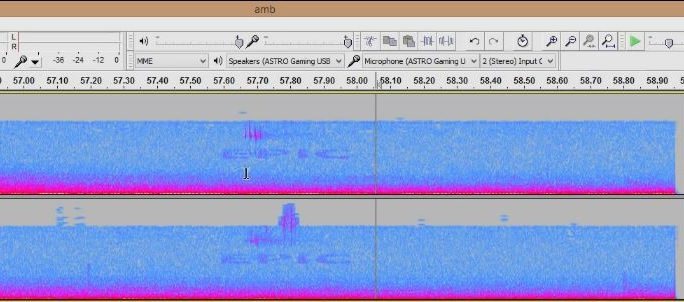
\includegraphics[width=7.7cm,keepaspectratio]{pics/audio_chapter/spectrogram_encoding.jpg}
    \caption{Message within the spectrogram viewed using Audacity.}
    \label{battlefield_spectrogram_easter_egg}
\end{figure}


\section{The MPEG-1/2 Audio Layer III (MP3)}
TO DO: research the MP3 format, how they store the audio samples, headers, compression, why it became so popular etc.

\section{Waveform Audio (WAV)}
The Waveform Audio format commonly known as WAV is a popular file format for storing high quality digital audio files originally built by Microsoft. It bears many similarities to the PNG format in the internal structure/composition of the file: both begin with a very specific sequence of bytes (also known as the magic bytes) that help classification applications identify them, are separated into multiple parts (also known as chunks) that have their purpose and are extremely common in the modern day multimedia.

TO DO: talk about the structure of the WAV format and the support for the steganography algorithms aforementioned.
\end{multicols}